\documentclass[11pt]{article}

%\usepackage{fullpage}
\usepackage[margin=1in]{geometry}
\usepackage{epsfig, hyperref}
%\usepackage{mathptmx}
\usepackage{algorithm}
\usepackage{algpseudocode}
\usepackage{times}
\usepackage{tabularx}
\usepackage{amsmath, amsthm, amssymb}
\usepackage{tikz}
\newtheorem{theorem}{Theorem}
\newtheorem{claim}{Claim}
\newcommand{\eat}[1]{}

\newcommand{\cI}{{\cal I}}
\newcommand{\cA}{{\cal A}}
\newcommand{\cB}{{\cal B}}
\newcommand{\bigO}{{\cal O}}
\newcommand{\opt}{{\mathsf{opt}}}
\usepackage{color}
\newcommand{\alert}[1]{\textcolor{red}{#1}}
\newcommand{\poly}{{\rm poly}}
\newcommand{\cR}{{\mathsf{CR}}}
\newcommand{\mk}{{\textsc{MARKING }}}
\newcommand{\expt}[1]{{\mathbb E[#1]}}
\newcommand{\prob}[1]{{\mathbb P[#1]}}

\title{
    \textbf{CSE586: Algorithms Under Uncertainty} \\
    Homework 2 Solutions % \\
    % Team Member 1: \href{mailto:ashlesha21380@iiitd.ac.in}{Ashlesha Gupta (2021380)} \\
    % Team Member 2: \href{mailto:divyajeet21529@iiitd.ac.in}{Divyajeet Singh (2021529)}
}
\author{
    \href{mailto:ashlesha21380@iiitd.ac.in}{Ashlesha Gupta (2021380)} \and
    \href{mailto:divyajeet21529@iiitd.ac.in}{Divyajeet Singh (2021529)}
}
\date{}

\begin{document}
\maketitle

\section*{Solution 1.}

\subsection*{Part (a)}
We are given a cycle graph of $n$ vertices. The given algorithm (let's say
$\mathbf{\Lambda}$) breaks the cycle by removing an arbitrary (but fixed) edge. To show that the competitive ratio
of the $\mathbf{\Lambda}$ is $\Omega(n)$, we simply provide an example where it performs
$n$ times worse than an offline optimal algorithm. \\
Consider a cycle graph of $n$ vertices with $k = 2$. We label the vertices in order
as $v_{1}, v_{2}, \ldots, v_{n}$. Without loss of generality, let's say $\mathbf{\Lambda}$ removes the edge $(v_{n}, v_{1})$. So, we have the following scenario.
\begin{figure}[htpb]
    \centering
    \begin{minipage}{0.4\textwidth}
        \centering
        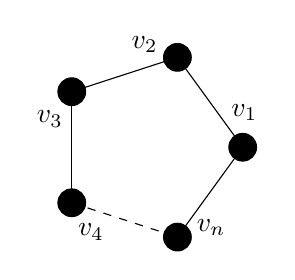
\begin{tikzpicture}
            \foreach \i in {1, ..., 5} {
                \coordinate (v\i) at ({72 * (\i - 1)}:1.2cm);
                \draw[fill=black] (v\i) circle (5pt);
                \ifnum \i=5
                    \node[draw=none,fill=none] at ({72 * (\i - 1)+20}:1.3cm) {$v_{n}$};
                \else
                    \node[draw=none,fill=none] at ({72 * (\i - 1)+20}:1.3cm) {$v_{\i}$};
                \fi
            }
            \foreach \i in {1, ..., 5} {
                \pgfmathtruncatemacro{\j}{mod(\i, 5) + 1}
                \ifnum \i=4
                    \draw[dashed] (v\i) -- (v\j);
                \else
                    \draw (v\i) -- (v\j);
                \fi
            }
        \end{tikzpicture}
    \end{minipage}
    \begin{minipage}{0.4\textwidth}
        \centering
        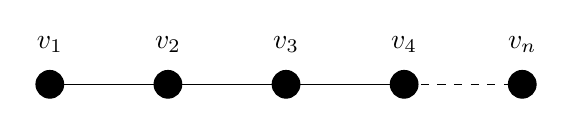
\begin{tikzpicture}
            \foreach \i in {1, ..., 5} {
                \coordinate (v\i) at ({1.5*\i-1}, 0);
                \draw[fill=black] (v\i) circle (5pt);
                \node[draw=none,fill=none] at (v\i) {\i};
                \ifnum \i=5
                    \node[draw=none,fill=none] at ({1.5*\i-1}, 0.5) {$v_{n}$};
                \else
                    \node[draw=none,fill=none] at ({1.5*\i-1}, 0.5) {$v_{\i}$};
                \fi
            }
            \foreach \i in {1, ..., 4} {
                \pgfmathtruncatemacro{\j}{\i + 1}
                \ifnum \i=4
                    \draw[dashed] (v\i) -- (v5);
                \else
                    \draw (v\i) -- (v\j);
                \fi
            }
        \end{tikzpicture}
    \end{minipage}
    \caption{Graphs used by the optimal and the given algorithm.}
\end{figure}
\vspace*{5pt} \\
Let the servers be initially located at the vertices $v_{1}$ and the \textit{middle}
vertex\footnote{If $n$ is odd, the middle vertex is $v_{\frac{n+1}{2}}$ and if $n$ is even, the middle vertex is $v_{\frac{n}{2}}$.}
$v_{\frac{n}{2}}$. An adversary can take advantage of the knowledge of the removed
edge - consider the input sequence $\sigma = \langle v_{1}, v_{n}, v_{\frac{n}{2}}, v_{1}, v_{n}, v_{\frac{n}{2}}, \ldots \rangle$.
Let us analyze the cost incurred by both the algorithms on $\sigma$. \\
Evaluate the performance of $\mathbf{\Lambda}(\sigma)$. First, the server at $v_{1}$ stays.
To serve the request at $n$, a server must move from $v_{\frac{n}{2}}$ to $v_{n}$, incurring a cost of $\frac{n}{2}$. Then, by
the double cover algorithm, both the servers move to the \textit{middle}\footnote{When $n$
is odd, both servers move to $v_{\frac{n+1}{2}}$, and otherwise, one server moves to
$v_{\frac{n}{2}}$ and the other moves to $v_{\frac{n}{2} + 1}$.} incurring a cost of $2 \cdot \frac{n}{2} = n$.
After this, each request at $v_{1}$ and $v_{n}$ costs $\frac{n}{2}$ (since before this, these servers must
be in the middle), and each request at $v_{\frac{n}{2}}$ costs $n$, since a request in the
middle forces both servers to jump to the middle. So, we have the total cost
\begin{align}
    \mathbf{\Lambda}(\sigma) &= \left( 0 + \frac{n}{2} + n \right) + \frac{|\sigma| - 3}{3} \cdot \left( \frac{n}{2} + \frac{n}{2} + n \right) \\
    &\leq \frac{|\sigma|}{3} \cdot \left( \frac{n}{2} + \frac{n}{2} + n \right) = \frac{2n|\sigma|}{3}
\end{align}
In contrast to this, the optimal algorithm $\mathbf{OPT}$, working on a circle, can keep
one circle to alternate between $v_{1}$ and $v_{n}$, and the other circle to stay fixed
at $v_{\frac{n}{2}}$. So, the cost incurred by $\mathbf{OPT}(\sigma)$ is
\vfill
\begin{align}
    \mathbf{OPT}(\sigma) &= \left( 0 + 0 + 1 \right) + \frac{|\sigma| - 3}{3} \cdot \left( 1 + 0 + 1 \right) \\
    &\leq \frac{|\sigma|}{3} \cdot \left( 1 + 0 + 1 \right) = \frac{2|\sigma|}{3}
\end{align}
Thus, we have the competitive ratio
\begin{align}
    \frac{\mathbf{\Lambda}(\sigma)}{\mathbf{OPT}(\sigma)} = \frac{2n|\sigma|}{3} \cdot \frac{3}{2|\sigma|} = n
\end{align}
Hence, the competitive ratio of the given algorithm is at least $\Omega(n)$.

\subsection*{Part (b)}
The given algorithm (let's say $\mathbf{\Lambda}$) breaks the cycle by removing any edge
uniformly randomly and performs the double cover algorithm on the resulting line. We need to prove
that $\mathbf{\Lambda}$ is $\bigO(k)$-competitive. \\
The expected cost of $\mathbf{\Lambda}$ on any input sequence $\sigma$ will be
\begin{equation}
    \label{eq:exp-cost}
    \mathbb{E}[\mathbf{\Lambda}(\sigma)] = \sum_{i=1}^{n} \frac{1}{n} \cdot \mathbf{\Lambda}_{i}(\sigma)
\end{equation}
where $\mathbf{\Lambda}_{i}$ is the algorithm that breaks the cycle by removing the edge $(v_{i}, v_{i+1})$,
for $i = 1, 2, \ldots, n-1$ and $(v_{n}, v_{1})$ for $i =  n$, and then performs the double cover algorithm on the resulting line.
Let the line formed by $\mathbf{\Lambda}_{i}$ be $l_{i}$. \\
There is an equivalent view point of \eqref{eq:exp-cost}. The cost paid by each line $l_{k}$ is weighed by $\frac{1}{n}$.
It is equivalent to say that for each requested vertex $\sigma_{j} (1 \leq j \leq |\sigma|)$, we move $\left(\frac{1}{n}\right)^{th}$ of a server from each line to the requested vertex.
For the lines $l_{k}$ where the requested vertex is between two serves (i.e. double coverage applies), it is
implicit that $\left(\frac{1}{n}\right)^{th}$ of at most 2 servers will be moved to $\sigma_{j}$, i.e.
the total movement is $2 \cdot \left(\frac{1}{n}\right)$ in some sense. \\
The analysis of this point of view of the algorithm will be done in a similar way as the analysis of the
double coverage algorithm covered in class. We define a non-negative potential function $\Phi$ such that
when the optimal algorithm $\mathbf{OPT}$ makes a move (incurs a cost $x$), $\Delta \Phi \leq 2k \cdot x$,
and when $\mathbf{\Lambda}$ incurs a cost $x$, the difference is $\Delta \Phi \leq -x$.
We define
\begin{equation}
    \label{eq:potential}
    \Phi = 2k \Psi + \Theta
\end{equation}
where $\Psi$ is the weighted distance between the servers of $\mathbf{OPT}$ and $\mathbf{\Lambda}$ and $\Theta$ is the
weighted sum of the distances of pairs of servers of $\mathbf{\Lambda}$ weighted by the fractions they move. It is easy to
see that $\Psi$ changes only when $\mathbf{OPT}$ makes a move, and changes only by integer amounts, since
$\mathbf{OPT}$ moves a server from one vertex to another.
\begin{align}
    \Psi &= \sum_{i=1}^{k} d(s_{i}^{*}, s_{i}) \cdot w_{s_{i}} \\
    \Theta &= \sum_{\text{unique } (s_{i}, s_{j})} d(s_{i}, s_{j}) \cdot w_{s_{i}} \cdot w_{s_{j}}
\end{align}
where $s_{i}^{*}$ is the location of the $i^{th}$ server of $\mathbf{OPT}$, $s_{i}$ is the location of the $i^{th}$ server of $\mathbf{\Lambda}$,
and $w_{s_{i}}$ is the weight of servers at $s_{i}$. So, $\Psi$ measures the cost of moving one server in $\mathbf{OPT}$. \\
Let's say $\mathbf{OPT}$ incurs a cost $x$ when it makes a move. Then, $\Theta$ remains unchaged. However,
$\Psi$ can increase by at most $x$. This is because $\mathbf{OPT}$ moves a server from one vertex to another, so, the
weighted distance between the servers of $\mathbf{OPT}$ and $\mathbf{\Lambda}$ can increase by at most $x$. In this case,
the potential difference is $\Delta \Phi \leq 2k \cdot x$, i.e. the potential increases by at most $2k \cdot x$. \\
Now, let's say $\mathbf{\Lambda}$ incurs a cost $x$. There can be two cases for each of the $n$ lines. Either the requested
vertex will lie to the extreme left or right of the line, or it will lie between two servers. \\
Let's say that the requested
lies to the extreme sides of $p$ out of the $n$ lines. Then, there are $p$ lines on which a server moves from one vertex to
another with a weight of $\frac{1}{n}$. $x$ is the total distance moved to serve the request, so $\Psi$ decreases by at most
$\frac{p}{n} \cdot x$ (because $p$ servers move by $x \cdot \frac{1}{n}$ each). Also, $\Theta$ increases by $\frac{p}{n} (k - \frac{p}{n}) \cdot x$,
because the distance of the $p$ servers moved from the other $k - \frac{p}{n}$ servers increases by $x \cdot \frac{p}{n}$ each. So, the potential
difference in total is
\begin{align}
    \Delta \Psi_{p} &\leq -\frac{p}{n} \cdot x \\
    \Delta \Theta_{p} &\leq \frac{p}{n} \left( k - \frac{p}{n} \right) \cdot x = k x \cdot \frac{p}{n} - x \cdot \frac{p^{2}}{n^{2}} \\
    \implies \Delta \Phi_{p} &= 2k \cdot \Delta \Psi_{p} + \Delta \Theta_{p} \\
    &= -2k \cdot x \cdot \frac{p}{n} + k \cdot x \cdot \frac{p}{n} - x \cdot \frac{p^{2}}{n^{2}} \\
    &\leq -2k \cdot x \cdot \frac{p}{n} + 2k \cdot x \cdot \frac{p}{n} - 2x \cdot \frac{p^{2}}{n^{2}} \\ %\quad \text{since } \frac{p^{2}}{n^{2}} \leq \frac{p}{n}\\
    \label{eq:diff-1}
    &= -2x \cdot \frac{p^{2}}{n^{2}}
\end{align}
At the same time, there are $n - p$ on which the requested vertex lies between two servers. On these lines, the servers move $\frac{2}{n}$ each
by the property of double coverage - 2 servers are moving $\frac{1}{n}$ on each line. In this case,
$\Psi$ either decreases or remains the same. This can be understood by realizing that the distance that increases by the servers on the left
of the requested vertex is the same as the distance that decreases by the servers on the right of the requested vertex, and vice versa. So,
$\Delta \Psi \leq 0$. On the other hand, if the total distance moved is $x$, and 2 servers move $\frac{1}{n}$ each, then $\Theta$ decreases by
$\left( \frac{n-p}{n} \right)^{2} \cdot x$. This is because the the total weight of the servers moved is $\left(\frac{n-p}{n}\right)^{2}$, and
$x$ is the total distance moved.
So, the potential difference is
\begin{align}
    \Delta \Psi_{n-p} &\leq 0 \\
    \Delta \Theta_{n-p} &\leq -\left( \frac{n-p}{n} \right)^{2} \cdot x \\
    \implies \Delta \Phi_{n-p} &= 2k \cdot \Delta \Psi_{n-p} + \Delta \Theta_{n-p} \\
    &\leq - \left( \frac{n-p}{n} \right)^{2} \cdot x
\end{align}
So, the overall potential difference is
\begin{align}
    \Delta \Phi &= \Delta \Phi_{p} + \Delta \Phi_{n-p} \\
    &= -2x \cdot \frac{p^{2}}{n^{2}} - \left( \frac{n-p}{n} \right)^{2} \cdot x \\
    &= -\frac{x}{n^{2}} \left( 2p^{2} + p^{2} + n^{2} - 2np \right)
\end{align}
When $p = 0$, $\Delta \Phi = -\frac{x}{n^{2}} \cdot n^{2} = -x$. When $p = n$, $\Delta \Phi = -\frac{x}{n^{2}} \cdot 2n^{2} = -2x$. Clearly,
$-2x \leq \Delta \Phi \leq -x$ when $\mathbf{\Lambda}$ makes a move. \\
We have proved that $\Delta \Phi \leq 2k \cdot x$ when $\mathbf{OPT}$ incurs a cost $x$ and
$-2x \leq \Delta \Phi \leq -x$ when $\mathbf{\Lambda}$ incurs a cost $x$.
The existence of this potential function $\Phi$ proves that $\mathbf{\Lambda}$ is $\bigO(k)$-competitive.


\section*{Solution 2.}

\subsection*{Part (a)}
We are required to follow a greedy strategy to maintain a maximum-size subset of disjoint
intervals while selecting intervals whose lengths are in $[2^{l}, 2^{l+1})$ for
some non-negative integer $l$.
\begin{claim}
    The greedy algorithm, let's say $\mathbf{\Lambda}$, for picking intervals of
    length $[2^{l}, 2^{l+1})$ is $\mathbf{\frac{1}{3}}$-competitive.
\end{claim}
\begin{proof}
    To prove the claim, we only need to show that for any input
    sequence $\sigma$,
    \begin{equation}
        \label{eq:cr-greedy}
        \frac{\mathbf{\Lambda}(\sigma)}{\mathbf{OPT}(\sigma)} \geq \frac{1}{3}
    \end{equation}
    where $\mathbf{ALG}(\sigma)$ represents the size of the subset of intervals picked by the algorithms
    on an input seqeunce $\sigma$.
    It is easy to see that picking smaller intervals is \textit{better}. Since $\mathbf{\Lambda}$
    picks greedily, every time it selects an interval, it potentially blocks upto 3 smaller intervals
    that $\mathbf{OPT}$ would select.
    In the worst case, $\mathbf{\Lambda}$ selects one interval of length $2^{l+1}-1$ while
    $\mathbf{OPT}$ picks 3 intervals of length $2^{l}$ each. This may happen for some $k \leq \frac{|\sigma|}{3}$ times, where each time,
    $\mathbf{\Lambda}$ picks a subset and blocks three subsets of \textit{half} the size. So, we have
    \begin{equation}
        \frac{\mathbf{\Lambda}(\sigma)}{\mathbf{OPT}(\sigma)} = \frac{k}{3 \cdot k} = \frac{1}{3}
    \end{equation}
    This proves that the claim in \eqref{eq:cr-greedy}.
\end{proof}


\section*{Solution 3.}

\subsection*{Part (a)}
We need to modify the exponential update algorithm to show a competitiveness of $\bigO(\log{f_{\max}})$
where $f_{\max}$ is the \textit{maximum} number of subsets to which any element can belong.
Our proposed algorithm is given in \ref{alg:exp-update}.
\begin{algorithm}
    \caption{A $\bigO(\log{f_{\max}})$ Exponential Update Algorithm for Fractional Set Cover}
    \label{alg:exp-update}
    \begin{algorithmic}[1]
        \State $f_{S} \gets 0 \quad \forall S \in \mathcal{F}$
        \While {elements $e \in U$ are arriving}
            \State If all sets $S_{e} : e \in S_{e}$ have $f_{S_{e}} = 0$, then $f_{S_{e}} \gets \frac{1}{f_{\max}} \quad \forall S_{e} : e \in S_{e}$
            \State If $\exists S^{*} : e \in S^{*}$ with $f_{S^{*}} \neq 0$, then $f_{S_{e}} \gets \left(\frac{1}{f_{\max}}\right)^{t+1}$
            $\quad \forall S_{e} : e \in S_{e}, f_{S_{e}} = 0$ where $f_{S^{*}}$ was initialized to $\left(\frac{1}{f_{\max}}\right)^{t}$
            \While {$\sum\limits_{S: e \in S} f_{S} < 1$}
                \State $f_{S} \gets \min{ \{ 1, 2 f_{S} \} } \quad \forall S: e \in S$
            \EndWhile
        \EndWhile
    \end{algorithmic}
\end{algorithm}
Here is an explanation of the algorithm. \\
The algorithm maintains a fraction $f_{S}$ for each subset $S \in \mathcal{F}$, initialized to 0.
When an element $e$ arrives for the first time that has never been covered in any set, we set its fraction to
$\frac{1}{f_{\max}}$ for all the subsets $S_{e}$ that contain $e$. \\
If an element arrives that has already been covered (partially) in some subset, the algorithm
assigns a fraction of $\left(\frac{1}{f_{\max}}\right)^{t+1}$ to all the subsets $S_{e}$ that
contain $e$ and have $f_{S_{e}} = 0$, where $t$ is the power of $\frac{1}{f_{\max}}$ assigned
to the subset $S^{*}$ that contains $e$ and has $f_{S^{*}} \neq 0$. Then, the algorithm simply follows the exponential update rule of doubling. \\
Now, we prove that Algorithm \ref{alg:exp-update} is indeed $\bigO(\log{f_{\max}})$-competitive.
\begin{claim}
    Algorithm \ref{alg:exp-update} is $\bigO(\log{f_{\max}})$-competitive.
\end{claim}
\begin{proof}
    The proof is very simple. For simplicity, let's call the algorithm covered in class as
    $\mathbf{M}$ and the proposed algorithm as $\mathbf{\Lambda}$. The first modification is that the fractions $f_{S}$ assigned to each subset $S$ are initialized from 0,
    instead of $\frac{1}{m}$ as done in $\mathbf{M}$. \\
    The intuition behind the algorithm is that if some subset has already been given some weight before,
    then instead of giving more weight to incoming/newer sets, we can increase the weight given to the older sets
    by doubling them (and setting the newer ones to higher powers of $\frac{1}{f_{\max}}$). This
    makes sure that the older sets get covered first, covering the new element more \textit{quickly}. \\
    Similar to the proof covered in class, in each (inner) iteration of $\mathbf{\Lambda}$,
    the weights corresponding to all the subsets in which the element $e$ occurs will be doubled,
    which means that there cannot be any iteration in which no subset of $\mathbf{OPT}$ participates.
    Note that even if the element $e$ occurs in previous subsets, every subset would have been initialized
    to \textbf{at most} $\frac{1}{f_{\max}}$, and therefore, when we double them, there can be \textbf{at most}
    $\bigO(\log{f_{\max}})$ iterations.
\end{proof}
An initialization of all weights to $\frac{1}{f_{\max}}$ does not work because
\begin{align}
    1 &\leq f_{\max} \leq m \\
    1 &\geq \frac{1}{f_{\max}} \geq \frac{1}{m} \\
    \implies m &\geq m \cdot \frac{1}{f_{\max}} \geq 1
\end{align}
which means that the total initialized weight can exceed 1. As it is easy to see, once we start doubling,
we end up paying much more than an offline optimal algorithm.

\subsection*{Part (b)}
For the rounding scheme, we assume that we know the value of $f_{\max}$. Let the final
weights assigned to each subset $S$ by the algorithm $\mathbf{\Lambda}$ in Part (a) be $f_{S}$.
We multiply each $f_{S}$ by $f_{\max}$ to get a value. If this value exceeds/equals 1, we round this subset up to 1.
Otherwise, we round it down to 0. \\
Let us analyse this deterministic rounding scheme. The final integer set cover solution
will have a cost of
\begin{align}
    C &= \sum_{S \in \mathcal{F}} f_{S} \cdot f_{\max} = f_{\max} \sum_{S \in \mathcal{F}} f_{S} \\
    &\leq f_{\max} \cdot \bigO(\log{f_{\max}}) \cdot \mathbf{OPT}(\sigma) \quad \text{by the analysis in Part (a)} \\
    &= \bigO(f_{\max} \log{f_{\max}}) \cdot \mathbf{OPT}(\sigma)
\end{align}
Therefore, the cost paid by this rounding scheme is $\bigO(f_{\max} \log{f_{\max}})$.


\section*{Solution 4.}
The given cat and mouse game is analogous to the Online Paging Problem that was
discussed in class. The $n$ vertices of the graph represent the pages\footnote{The
terms \textit{vertex} and \textit{page} are used interchangeably in this solution.}.
The cache size can be assumed to be $n-1$. We say that the only page not in the cache
is the one that the mouse is currently on. The cat behaves as an online adversary
trying to hit a cache miss\footnote{By the problem definition, hitting a cache miss
does not mean that the cat catches the mouse - it simply means that the mouse
\textbf{must} move}. The mouse acts as the algorithm\footnote{The terms \textit{mouse}
and \textit{algorithm} are used interchangeably in this solution.} trying to minimize
its movement (i.e. the number of cache misses).

\subsection*{Part (a)}
Given the constraint that each move costs 1 when $m_{t+1} \neq m_{t}$, we propose
the following 1-bit marking algorithm for the mouse. We begin with all vertices
unmarked. At each time step $t$, when the cat moves to any vertex $c_{t}$, one of
two cases can arise:
\begin{enumerate}
    \item $c_{t} \neq m_{t-1}$, i.e. $c_{t}$ is \textit{in cache}. In this case,
    we simply mark the vertex if it is not already marked. The mouse stays on
    $m_{t} = m_{t-1}$.
    \item $c_{t} = m_{t-1}$, i.e. $c_{t}$ is a cache miss. In this case, we mark
    $c_{t}$ and the mouse moves to an arbitrary unmarked vertex $m_{t}$. If all
    vertices were marked, we unmark all of them and execute this step.
\end{enumerate}
By \textbf{Theorem 3.} in [1], the marking algorithm is $k$-competitive where
$k$ is the cache size. So, the proposed algorithm is $(n-1)$-competitive.

\subsection*{Part (b)}
We need to prove a claim similar to \textbf{Theorem 2.} in [1] for the given cat
and mouse game. \\
Let us fix any deterministic algorithm $\mathbf{A}$ for the mouse. Note that the
number of pages is fixed to $n$ and the cache size is $k = n-1$. This means that
there exists exactly one page at each time step, in our case, $m_{t-1}$, that is
not present in the cache. So, at every time step $t$, the cat can move to the vertex
$m_{t-1}$ (i.e. \textit{request for page $m_{t-1}$}), forcing the mouse
to move (to serve the cache miss), incurring a cost of 1 in each step. So, for an
input sequence $\sigma$, $\mathbf{A}$ suffers a cost of $|\sigma|$. \\
However, an offline optimal mouse (something similar to LFD for paging) knows in
advance the subsequent moves of the cat. So, for every cache miss, the optimal mouse
moves to a vertex $v$ where the cat would arrive the farthest in the future. The
cat will reach $v$ after at least $k-1$ or $n-2$ time steps. If the cat moves to $v$
before $n-2$ requests that were \textit{in the cache} when the mouse moved to $v$,
then it wouldn't be the farthest-in-the-future vertex, as there would be some other
vertex that is accessed later than $v$. Hence, the optimal mouse suffers a cost of at
most $\frac{|\sigma|}{n-1}$. \\
Thus, the competitive ratio of any deterministic algorithm $\mathbf{A}$ is at least
$n-1 = \Omega(n)$.

\subsection*{Part (c)}
Following the same argument as class notes, we propose the randomized marking
algorithm as an $\bigO(\log{n})$-competitive algorithm for the cat and mouse game.
The description of the algorithm is as follows:
\begin{enumerate}
    \item When the cat moves to a vertex $v_{t} \neq m_{t-1}$, the mouse stays at
    $m_{t} = m_{t-1}$ and marks $v_{t}$ if it is not already marked.
    \item Otheriwse, we mark $v_{t}$ and the mouse moves to an unmarked vertex $m_{t}$
    chosen uniformly at random. If all vertices are marked, we unmark all of them
    and execute this step.
\end{enumerate}
It is shown in \textbf{Theorem 4.} in [1] that the cost paid by an offline optimal
mouse is bounded below by
\begin{equation}
    \label{eq:opt-mouse}
    \mathbf{OPT}(\sigma) \geq \sum_{i=1}^{p} \frac{d_{i}}{2}
\end{equation}
where the mouse goes through $p$ many \textit{phases} and $d_{i}$ is the number of
vertices visited by the cat which are distinct from all the vertices visited by it in phase
$P_{i-1}$. Let $q_{i}$ be the number of times $c_{t} = m_{t-1}$, i.e.
the number of times the cat hits a cache miss in phase $P_{i}$. \\
Now we bound the expected number of cache misses suffered by randomized marking. It
is obvious that in each phase $P_{i}$, the randomized mouse suffers at least $d_{i}$
misses, since these are new requests which are not \text{in cache} at the beginning
of $P_{i}$. Other than these, there can be at most $n-1-d_{i}$ \textit{old} vertices
which the mouse may have visited (since they were unmarked at the beginning $P_{i}$)
but then the cat visits again in $P_{i}$. The mouse picks these vertices to visit randomly. \\
Let us call the old vertices $o_{1}, o_{2}, \ldots, o_{n-1-d_{i}}$ according to their order
of first visits by the cat in $P_{i}$. Define a random variable $X_{j}$ as follows
\begin{equation}
    X_{j} = \begin{cases}
        1 & \text{ if } o_{j} \text{ was a cache miss, i.e. the cat visited } o_{j} = m_{t-1} \\
        0 & \text{ otherwise}
    \end{cases}
\end{equation}
The total number of cache misses due to the \textit{old} vertices is $X$, the sum of all
$X_{j}$ for $j = 1, 2, \ldots, k-1=n-2$. So, the expected number of cache misses suffered by randomized marking is
\begin{equation}
    \mathbb{E}[X] = \mathbb{E} \left[ \sum_{j=1}^{n-2} X_{j} \right] = \sum_{j=1}^{n-2} \mathbb{E}[X_{j}]
    = \sum_{j=1}^{n-2} \mathbb{P}[X_{j} = 1] \quad \text{since } X_{j} \text{ are an indicator variables}
\end{equation}
Now, we bound the probability that each indicator variable takes the value 1. The mouse
will visit vertex $o_{1}$ because the cat visited its earlier vertex $m_{t-1}$. Let $\bar{n}_{1}$
be the number of vertices visited by the cat before its first visit to $o_{1}$ in $P_{1}$.
So, we select a subset of size $\bar{n}_{1}$ from $n-1$ old vertices uniformly at random.
So, the probability of $o_{1}$ being among these selected vertices is
\begin{equation}
    \frac{\bar{n}_{1}}{n-1} \leq \frac{d_{i}}{n-1}
\end{equation}
Similarly, let $n_{2}$ be the number of new vertices visited by the cat before its first visit to
$o_{2}$. However, the mouse may have already visited $o_{2}$ because it was forced to leave
vertex $o_{1}$ when the cat visited it. At this stage, the total number of unmarked pages is $n-2$,
since $o_{1}$ would have been marked. So, the probability of the cat visiting $o_{2}$ when the mouse
is at it becomes
\begin{equation}
    \frac{n_{2}}{n-2} \leq \frac{d_{i}}{n-2}
\end{equation}
Continuing this way, we get the probability of $o_{j} (j = 1, 2, \ldots, n-2)$ being a cache miss as
\begin{equation}
    \mathbb{P}[X_{j} = 1] \leq \frac{d_{i}}{n-1-j}
\end{equation}
Thus, we have the expected number of cache misses
\begin{equation}
    \mathbb{E}[X] = \sum_{j=1}^{n-2} \mathbb{P}[X_{j} = 1] = \sum_{j=1}^{n-2} \frac{d_{i}}{n-1-j}
    = d_{i} \cdot \bigO(\log{n})
\end{equation}
Then, adding up over all phases $P_{i}$ for $i = 1, 2, \ldots, p$, we get the upper bound on the
expected number of misses for a randomized mouse, which is
\begin{equation}
    \sum_{i=1}^{p}(d_{i} + d_{i} \cdot c \log{n}) \leq c \log{n} \cdot \sum_{i=1}^{p} d_{i} = \bigO(\log{n}) \cdot \mathbf{OPT}(\sigma)
\end{equation}
where the last inequality follows from the lower bound on $\mathbf{OPT}(\sigma)$ in \eqref{eq:opt-mouse}.
This proves that the proposed randomized marking algorithm is $\bigO(\log{n})$-competitive.


\section*{Solution 5.}
For the given randomized algorithm for vertex cover with online edge arrivals, we
need to prove that
\begin{equation}
    \mathbb{E}[\mathbf{\Lambda}(\sigma)] \leq 2 \cdot \mathbf{OPT}(\sigma)
\end{equation}
We try to estimate and bound the total expected cost paid by our algorithm on any input
sequence, as compared to an offline optimal algorithm which knows the input of edges. \\
It is clear that $\mathbf{OPT}$ may or may not select an edge at every time step $t \leq |\sigma|$.
So, let's say that $\mathbf{OPT}$ selects an edge at time steps $t_{1}, t_{2}, \ldots, t_{N}$
where $N \leq |\sigma|$ and $t_{i} < t_{i+1} \quad \forall i = 1, 2, \ldots, N-1$. Let the time
steps $[t_{i}, t_{i+1})$ define a \textit{phase}, say $P_{i}$, for every $i = 1, 2, \ldots, N-1$.
In each phase $P_{i}$, $\mathbf{OPT}$ makes only 1 selection. So, we prove that in expectation, the
number of vertices chosen by $\mathbf{\Lambda}$ in each phase is upper bounded by 2. \\
Let the number of vertices chosen in each phase $P_{i}$ be $S_{i}$. Then, we have
\begin{equation}
    \mathbb{E}[S_{i}] = \sum_{j=1}^{k} j \ \mathbb{P}[S_{i} = j]
    \quad \text{where } k = t_{i+1} - t_{i} \text{, the no. of time steps in } P_{i}
\end{equation}
\begin{claim}
    The probability that $\mathbf{\Lambda}$ chooses $j$ vertices in phase $P_{i}$ is
    \begin{equation}
        \mathbb{P}[S_{i} = j] = \frac{1 + \mathbb{I}_{\{j = k\}}}{2^{j}} = \begin{cases}
            \frac{1}{2^{j}} & j \neq k \\[5pt]
            \frac{2}{2^{j}} & j = k
        \end{cases}
    \end{equation}
    where $k$ is the number of time steps in phase $P_{i}$, i.e. $k = t_{i+1} - t_{i} $.
\end{claim}
\begin{proof}
    First, it is easy to see that the distribution of probabilities is valid, i.e. it sums to 1.
    This is because
    \begin{align}
        \sum_{j=1}^{k-1} \frac{1}{2^{j}} + \frac{2}{2^{k}} &= \sum_{j=1}^{k-1} \frac{1}{2^{j}} + \frac{1}{2^{k-1}} \\
        &= \sum_{j=1}^{k-2} \frac{1}{2^{j}} + \frac{2}{2^{k-1}} \\
        &= \cdots = \frac{1}{2} + \frac{2}{2^{2}} = 2 \cdot \frac{1}{2} = 1
    \end{align}
    Now, we prove the claim. \\
    Let $v^{*}$ be the vertex chosen by $\mathbf{OPT}$ in phase $P_{i}$. $\mathbf{\Lambda}$ picks
    any vertex of an input edge with half probability, which means that it picks $v^{*}$ at time
    $t_{i}$ with probability $\frac{1}{2}$. If it picks $v^{*}$, then it does not need to pick any other
    vertex till $t_{i+1}$, thereby matching $\mathbf{OPT}$. This means that $\mathbb{P}[S_{i} = 1] = \frac{1}{2^{1}}$. \\
    If $\mathbf{\Lambda}$ does not pick $v^{*}$ at $t_{i}$, then it picks $v^{*}$ at $t_{i} + 1$
    with half probability. This means that $\mathbb{P}[S_{i} = 2] = \frac{1}{2} \cdot \frac{1}{2} = \frac{1}{2^{2}}$.
    This continues till time\footnote{Simply put, everytime we choose something wrong, the probability
    decreases by half and the size of chosen set of vertices increases by 1.} $t_{i+1} - 2$, i.e. $\mathbb{P}[S_{i} = j] = \frac{1}{2^{j}}, 1 \leq j < t_{i+1} - 1$. \\
    At the last step of the phase, $t_{i+1} - 1$, it does not matter which vertex $\mathbf{\Lambda}$ picks; the size of
    the picked vertex set will be $k = t_{i+1} - t_{i} $. If it picks
    either, the phase ends anyway. So, there are two possibilities of making $S_{i} = k$. So,
    of $\mathbb{P}[S_{i} = k] = \frac{2}{2^{k}}$.
\end{proof}
Now we have
\begin{align}
    \mathbb{E}[S_{i}] &= \sum_{j=1}^{k} j \ \mathbb{P}[S_{i} = j] = \sum_{j=1}^{k-1} j \cdot \frac{1}{2^{j}} + k \cdot \frac{2}{2^{k}} \\
    &= \sum_{j=1}^{k} \frac{j}{2^{j}} + \frac{k}{2^{k}} \\
    &\leq \lim_{k \to \infty} \sum_{j=1}^{k} \frac{j}{2^{j}} + \frac{k}{2^{k}} = 2 + 0 = 2
\end{align}
where the summation is bounded by 2 (sum of arithmetico-geometric series, given in \eqref{eq:ags}), and the other
limit is trivially true (exponential grows faster than linear). \\
\begin{equation}
    \label{eq:ags}
    \sum_{j=1}^{\infty} j \cdot \frac{1}{2^{j}} = \frac{\frac{1}{2}}{(1 - \frac{1}{2})^{2}} = \frac{1}{2} \cdot \frac{4}{2} = 2
\end{equation}
We have proved that in each phase, if $\mathbf{OPT}$ selects one vertex, then $\mathbf{\Lambda}$ selects at most 2 vertices
in expectation. Summing over all $N$ phases, we get
\begin{equation}
    \mathbb{E}[\mathbf{\Lambda}(\sigma)] = \sum_{i=1}^{N} \mathbb{E}[S_{i}] \leq \sum_{i=1}^{N} 2 = 2 \cdot N \leq 2 \cdot \mathbf{OPT}(\sigma)
\end{equation}
where the last inequality holds because $\mathbf{OPT}$ picks one vertex in each of the $N$ phases by definition. This proves that the given randomized
algorithm is $\mathbf{2}$-competitive.


\section*{References}
\begin{enumerate}
    \item \href{https://drive.google.com/file/d/1XNEFcQVAwPxwWcIc7JNnV_KkknwTE8le/view}{Lecture Notes on Online Paging, CSE586 (Monsoon 2023, Dr. Syamantak Das)}
    \item \href{https://drive.google.com/file/d/1oiCLx6IrV6MFVn__o1-i53MMMUvXgmof/view}{Lecture Notes on Online Computation \& Network Algorithms, CS294-1 (Spring 1997, Yair Bartal)}
    \item \href{https://sci-hub.se/https://link.springer.com/article/10.1007/BF01189994}{A Deterministic $\bigO(k^{3})$-competitive $k$-Server Algorithm for the Circle, A. Fiat et al.}
    \item \href{https://people.cs.uchicago.edu/~duru/papers/masters.pdf}{The $k$-Server algorithm and Fractional Analysis, Duru Turkoglu}
    \item \href{https://en.wikipedia.org/wiki/Arithmetico-geometric_sequence}{Wikipedia - Arithmetico-Geometric Series}
\end{enumerate}

\end{document}